\documentclass{article}
\usepackage{tikz}
\usepackage{graphicx}
\usetikzlibrary{shapes.geometric}
\usetikzlibrary{external}
\tikzexternalize[mode=list and make] % !activate

\tikzset{
    % Defines a custom style which generates BOTH, .pdf and .png export
    % but prefers the .png on inclusion.
    %
    % This style is not pre-defined, you may need to copy-paste and
    % adjust it.
    png export/.style={
        external/system call/.append=
            {; convert -density 300 -transparent white "\image.pdf" "\image.png"}
        %
        %/pgf/images/external info,
        %/pgf/images/include external/.code={%
        %    \includegraphics
        %        [width=\pgfexternalwidth,height=\pgfexternalheight]
        %        {##1.png}%
        %},
    }
}
\tikzset{png export}
\begin{document}


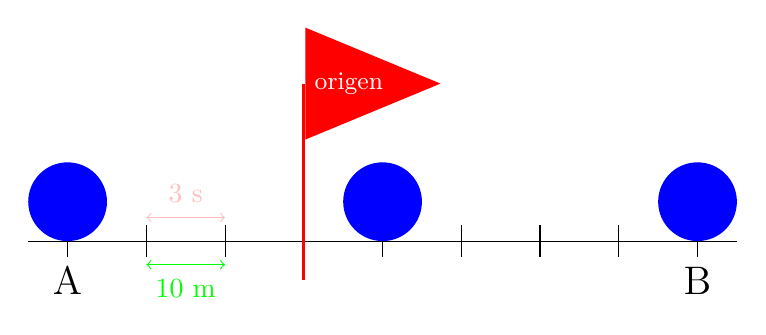
\begin{tikzpicture}[png export,scale=1]
    \draw (-3.5,0) -- (5.5,0);
    \foreach \x in {-3,-2,-1,1,2,3,4,5}
    \draw (\x,0.2) -- (\x,-0.2);
    \draw[red,very thick] (0,-0.5) -- (0,2) node[red,isosceles triangle,fill,anchor=west,text=white,font=\small] {origen};
    \node[font=\Large] (A) at (-3,-0.5) {A};
    \node[font=\Large] (B) at (5,-0.5) {B};
    \fill[blue] (-3,0.5) circle [radius=0.5];
    \fill[blue] (1,0.5) circle [radius=0.5];
    \fill[blue] (5,0.5) circle [radius=0.5];
    \draw[<->,pink] (-2,0.3) -- node[above=2pt] {3 s} (-1,0.3);
    \draw[<->,green] (-2,-0.3) -- node[below=2pt] {10 m} (-1,-0.3);
\end{tikzpicture}


\end{document}